% !TEX root = ../report.tex

\chapter{Preliminary Study}
% http://www-03.ibm.com/press/us/en/pressrelease/42451.wss

\minitoc
\noindent
This chapter studies various technologies, research and information that is relevant to the project goals.

Beyond this, the study will serve to outline which direction the project must take and what methodologies must be used. Since there span of possibilities and directions are broad and few studies with similar goals of sufficient quality and completeness exist, the study is lengthy and a large part of the project.

\clearpage

% \section{Set to work with (another name perhaps (or maybe completely removed))}
% About Netflix


\section{Netflix}
% http://en.wikipedia.org/wiki/Netflix
% http://blog.jimjh.com/static/downloads/2013/05/12/netflix.pdf

\begin{wrapfigure}{r}{.30\textwidth}
\vspace{-30pt}
\centering

\includegraphics[width = .25\textwidth]{image/netflix-logo.png}
\end{wrapfigure}
This is the prestudy for the movie recommendation part of the system. We will look into what Netflix is, at the datasets and its statistics, and how to explore it.

\subsubsection{About Netflix}
Netflix is a on-demand Internet streaming media. It started out as a DVD-rental business, but moved over to a more Internet based business model in 1999 and have from then on had a great success in the subscription-based digital distribution service. To improve customer satisfaction they developed a personalized video-recommendation system called Cinematch. About 60\% of the Neflix users select their next movie or TV-show based on this recommendation~\cite{hownetflixworks}, so it is important that this recommendation system manages to capture the users movie and TV-show preferences and feed back fitting movies and TV-shows.

\subsubsection{Cinematch}
\label{subsec:Cinematch}
% http://electronics.howstuffworks.com/netflix2.htm
This recommendation system is self-updating. It searches the Cinematch database for users who have rated the same movie, determents which of these again have rated a second movie and with this calculates likelihood that users who like the first also likes the second one.


\subsection{The Dataset}\label{subsec:netflixdata}
Netflix held a competition where the contest was made to help Netflix improve their movie recommendation system. The team that could beat Netflix's own collaborative filtering system by more than 10\% could win one million dollars. To measure the score root-mean-square error (RMSE) was used, which is used to measure the difference between the values predicted or estimated and the actual values observed. The RMSE of Cinematch~\ref{subsec:Cinematch} was at 0.9525.

\subsubsection{Root-mean-square error RMSE}\label{subsubsec:rmse}

\begin{equation}\label{eq:rmse}
RMSE = \sqrt {{\frac{{\sum\limits_{{i = 1}}^n {{{\left( {{y_i} - {{\hat{y}}_i}} \right)}^2}} }}{{n}}}}
\end{equation}

The equation for calculating the RMSE is show in figure~\ref{eq:rmse}. It calculates how far the estimated value is from the actual value. Here ${y_i}$ is the actual value and ${\hat{y}}$ is the estimated value. The square difference of all the values are averaged, where ${n}$ is the number of values, this result is rooted. This produces the average distance of all the estimate values from the all the actual values~\cite{rmse}.


\subsubsection{Competition}

For this competition Netflix produced a training dataset based on user ratings from their own database. It contains 100 480 507 ratings from 480 189 unique users on 17 770 movies. The data is split up into 17 770 files, one for each movie, where the data is a triplet of the form <user, rating, date-of-rating>. The user-field and rating-field is an integer, while the date-of-rating-field is on the ISO 8601 form, year-month-day. The different movies have different amounts of ratings, and the different users have rated different amounts of movies rated.

With the training dataset the teams system was supposed to predict ratings on a "qualifying"-dataset, which contained 2 817 131 triplets with only user ids, movie ids and dates. This "qualifying"-datase must be disregarded since the actual ratings for this dataset was only know to the jury of the competition and is nowhere to be found. Instead a probe set is provided with 1 408 385 users which can be used to remove these from the training set to test predictions based on the test set. This probe set possesses similar statistical values as the qualifying set, so it will give a good prediction of how the result actually would have scored in the competition\cite{nfprizeset}.

\begin{table}[H]
\centering
\begin{tabular}{ l l }
\hline
\textbf{Ratings} & 100 480 507 \\ \hline
\textbf{Customers} & 480 189 \\ \hline
\textbf{Movies} & 17 770 \\ \hline
\textbf{Qualifying set} & 2 817 131 \\ \hline
\textbf{Probe set} & 1 408 385 \\ \hline
\end{tabular}
\captionof{table}[Netflix-dataset statistics]{The data statistics from the dataset provided by Netflix in the Netflix Prize competition}\label{tab:nfDatasetStat}
\end{table}

\begin{figure}[H]
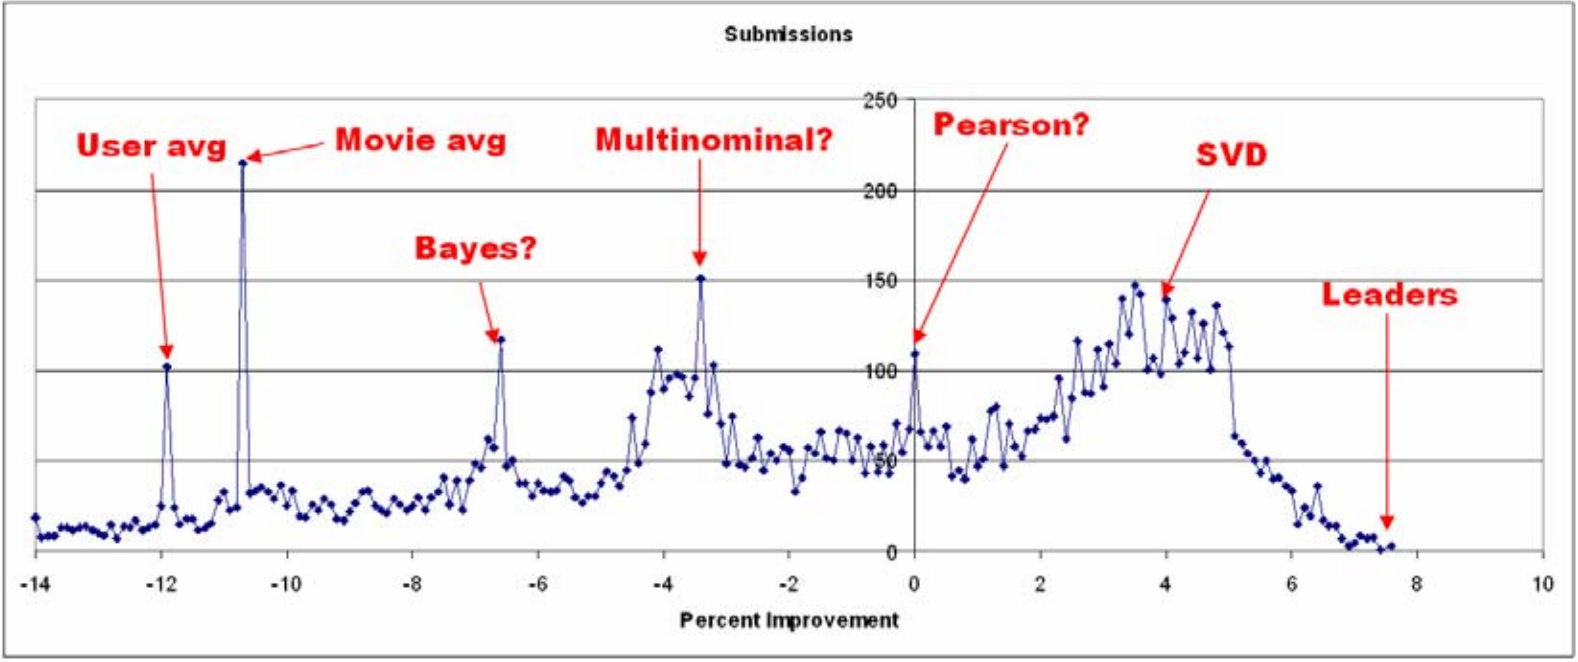
\includegraphics[width=5in]{image/sub-distr-nf.png}
\centering
\caption[Distribution of different submission]{Distribution of different submission amount, their score and the most used algorithms to produce the RMSE score. As we can see from the figure, one of the better performing algorithms are singular value decomposition (SVD). Approaches like using the average movie rating to suggest ratings and the average ratings for users, was often used, but did not produce a good recommendation (RMSE reduction from the Cinematch score by 10-12\%)}
\label{figure:sub-distr-nf}
\end{figure}

\subsubsection{Dataset statistics}
% http://en.wikipedia.org/wiki/Principal_components_analysis
% http://en.wikipedia.org/wiki/Singular_value_decomposition
% http://en.wikipedia.org/wiki/Latent_semantic_indexing
% http://www.timelydevelopment.com/demos/NetflixPrize.aspx

To better understand the dataset, some statistics about the dataset was produced.

\begin{figure}[H]
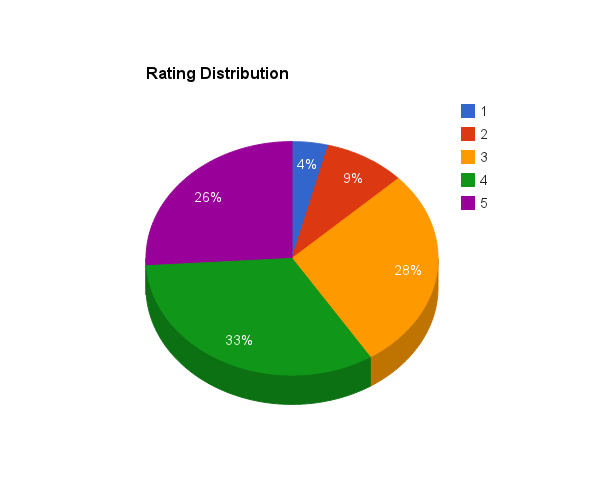
\includegraphics[width=5in]{image/ratingdistr.png}
\centering
\caption{Rating distribution}
\label{figure:ratingdistr}
\end{figure}

Rating distribution is shown in figure~\ref{figure:ratingdistr}. 1/3 of the ratings are 4, and rating 1 and 2 only makes up for 13\% of the rating distribution. 3 and 5 are quite similarly represented with 28\% and 26\% respectively. It can from this be assumed a greater prediction towards the higher ratings, and predictions towards lower ratings should not be done lightly.

\begin{figure}[H]
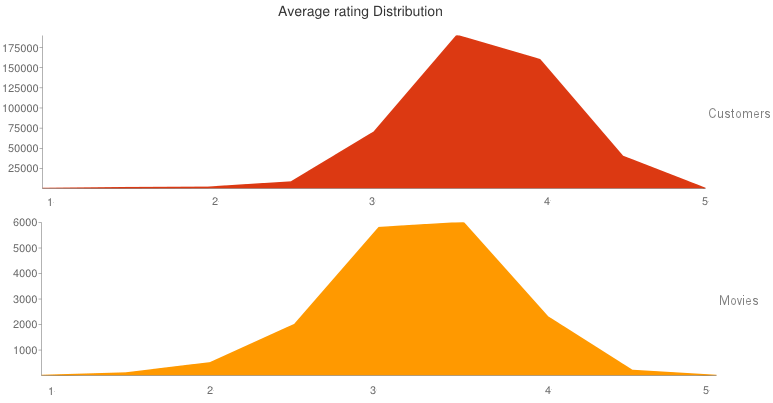
\includegraphics[width=5in]{image/avgratingdistr.png}
\centering
\caption{Average rating distribution}
\label{figure:avgratingdistr}
\end{figure}

Average rating distribution is shown in figure~\ref{figure:avgratingdistr}. The red(upper) graph shows average rating distribution of the customers, while the orange(bottom) one shows the distribution per movie. Both graphs have quite similar form. Both customers and movies peak at a rating of 3,5, which is natural. The second highest point is for the customers at 4, and for the movies at 3. The actual average user rating of all movies is closer to 3.7.

\begin{figure}[H]
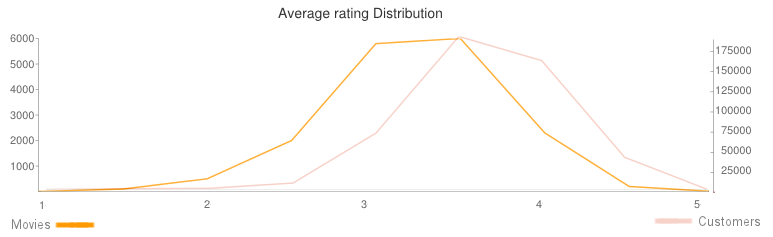
\includegraphics[width=5in]{image/avgratdistrover.png}
\centering
\caption{Average rating distribution}
\label{figure:avgratdistrover}
\end{figure}


\begin{figure}[H]
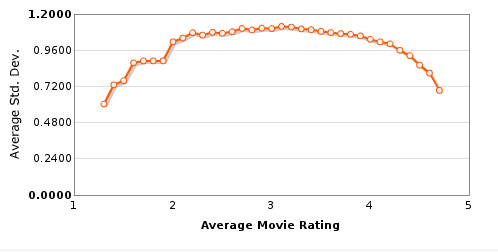
\includegraphics[width=5in]{image/avgmovierating.png}
\centering
\caption{Average movie rating distribution~\cite{td-nf-r}}
\label{figure:avgmovierating}
\end{figure}

Average movie rating distribution is shown in figure~\ref{figure:avgmovierating}. Here we see that for the edge ratings (rating 1 or 5) has the least standard deviation, so when a movie is highly rated it usually is rated high, and the same goes for low ratings, while for the middle ratings (2 to 4) we see that it variates more, and quite similarly. So the middle ratings are harder to classify, in other words, when a movie has a rating of 3, the average rating-shift is almost 1.1.
% End Netflix



% About Weka
\section{Weka}
%http://en.wikipedia.org/wiki/Weka_(machine_learning)

\begin{wrapfigure}{r}{.30\textwidth}
\vspace{-30pt}
\centering

\includegraphics[width = .25\textwidth]{image/Weka-logo.png}
\end{wrapfigure}


Weka is a machine learning software written in Java. It can be used to visualize data through analyzing it with different kinds of algorithms. The Explorer, a graphical user interface, makes it easy to work with and explore data from different angles. It is a free software under the General Public License \cite{GNU}. Weka can handle several data mining tasks, including, data preprocessing, clustering, classification, regression and feature selection. The input data has to be a single flat file or relation, each data point must be described by a fixes number of attributes. The dataset can be accessed trough a SQL database. Can link database tables into a single datatable, which can be used for processing using Weka.


\subsection{ARFF}
% http://www.cs.waikato.ac.nz/ml/weka/arff.html
Attribute Relationship File Format is the file type used to store data in a database. The structure is as follows:

\begin{lstlisting}[caption={ARFF Example},label={lst:arffEx},captionpos=b]
@relation 'flat-netflix'

@attribute assetId string
@attribute 14367 numeric
@attribute 6050 numeric
@attribute 14112 numeric

@data
1658496,?,?,4
684232,3,3,?
684231,4,?,?
1774519,1,?,?
\end{lstlisting}

Listing~\ref{lst:arffEx} is an example of how an ARFF file is structured. It startes with a header, containing "@relation", "@attribute"s and the "@data". This header defines the name of the relation, the attributes in the dataset and the data. The "@data"-header contains arrays, where each array has values for the corresponding "@attribute"s values. If a array has no value for a particular attribute it is denoted as a question mark (?).

\subsection{The Explorer}
% http://www.cs.waikato.ac.nz/~ml/weka/gui_explorer.html
% http://research.cs.queensu.ca/home/cisc333/tutorial/Weka.html
% http://wiki.pentaho.com/display/DATAMINING/Time+Series+Analysis+and+Forecasting+with+Weka
\begin{table}[H]
\centering
\begin{tabularx}{1.0\textwidth}{ l p{9.3cm} }
  \textbf{Components} & \textbf{Description} \\
  \hline \\ [-1.5ex]
  Preprocess & Here the user can import the data which is going to be analyzed. It is also possible to do some filtering on this data, this includes removing of values and transforming values. \\
  \hline \\ [-1.5ex]
  Classify & Here the user can apply classification and regression algorithms to the dataset. \\
  \hline \\ [-1.5ex]
  Associate & Here the user can have the association rule learners identify important relationships between attributes in the provided dataset. \\
  \hline \\ [-1.5ex]
  Cluster & Here the user can apply cluster algorithms to the dataset \\
  \hline \\ [-1.5ex]
  Select attributes & Here the user can identify the most predictive attributes in the dataset. \\
  \hline \\ [-1.5ex]
  Visualize & Here the user can get a visualization of the dataset, and of the different algorithms preformed on the dataset. \\
\end{tabularx}
\caption{Classification based on feature}
\label{table:nosql-calssifications}
\end{table}

\subsection{Machine-learning algorithms}
Weka can let the user utilize its many machine-learnings algorithms in an easy and convenient way. It opens for easy implementations of the algorithms though both just input of a file and get a result back, or though incorporating the algorithms in code.
% End Weka




% About Twitter
\section{Twitter}\label{sec:twitter}

\begin{wrapfigure}{r}{.30\textwidth}
\vspace{-30pt}
\centering

\includegraphics[width = .25\textwidth]{image/twitter-logo.png}
\end{wrapfigure}
Twitter is a free social media network based on microblogging. In microblogging, a user can post a paragraph of a certain number of characters or less to his/her timeline. The user can also follow other users. Whenever the users that a given user is following posts something, the user can see these posts in his/her feed. This is the basis for many of todays most popular social media networks, including Twitter.

\subsection{Terminology}
For more clarity, we define the terminology twitter uses. All words in \textbf{bold} are our own definitions for more easily describing how the various term relate to eachother.

\subsubsection{Tweet}
A tweet is a post containing max 140 characters. It can also refer to the verb ‘to tweet’, which means ‘to post a tweet’. \textbf{tweets} is an attribute of a user which returns a list of tweets that the users

  \textbf{user.tweets -> [<tweet>]}
\subsubsection{User}
A user is someone with a twitter account. A user can post tweets. By following other users, twitter generates a feed for the user containing the tweets of all the users they follow. They also have certain information retrieval tools available, such as filtering tweets by a tag name, specific user or search term.

\subsubsection{Tweeter}
A user who tweets a tweet that is referenced in the same context. For instance: The best tweets are tweeted by the most popular tweeters


\subsubsection{Follower}
A follower is someone who follows a user. The follower will see the users tweets in their feed. \textbf{followers} is an attribute of a user which returns the list of users that are following that user.

  \textbf{user.followers -> [<user>]}

\subsubsection{Followee}
A followee is someone who a user is following. The user will appear in the followees list of followers, and the followee will appear in the users list called ‘following’. We will refer to the list ‘following’ for a user as followees for clearer terminology. \textbf{followees} is an attribute of a user which returns the list of users that the user is following.

  \textbf{user.followees -> [<user>]}

\subsubsection{Hashtag}
Hashtags are topic labels that are placed on tweets. They are made by typing \#topicname anywhere in the tweet. By navigating to \#topicname, a user will see a feed of all tweets containing \#tagname. \textbf{hashtags} is a an attribute of a tweet which returns the list of hashtags the tweet contains.

  \textbf{tweet.hashtags -> [<hashtag>]}

\noindent
Hashtag also has the attribute tweets, which returns all tweets that have a certain hashtag. These hashtags are ordered by twitters algorithm which balances how recent the tweet is with the popularity of the tweeter.

  \textbf{hashtag.tweets -> [<tweet>]}

\subsubsection{Usertag}
Usertags are labels that are placed on tweets describing who the tweets are adressed to. They are made by typing @username anywhere in the tweet. This tweet will also show up in the feed of the user with name username. \textbf{usertags} is an attribute of a tweet which returns the list of users that the tweet is adressed to.

\textbf{tweet.usertags -> [<user>]}

\subsection{Legal Considerations}\label{sec:pre-twitter-legal}
Collect and use a data set from twitter, a company whose currency is information, must be done in a way that complies with their rules and terms of service. This section considers how an automated system can collect information from twitter and what an automated system can use it for.

\subsubsection{API Terms}
You may use the Twitter API and Twitter Content in connection with the products or services you provide (your "Service") to search, display, analyze, retrieve, view, and submit information to or on Twitter \cite{twitter-api-terms}. This means that data can be gathered within the limitations set by the API to gather a dataset and analyze it.

If you provide downloadable datasets of Twitter Content or an API that returns Twitter Content, you may only return IDs (including tweet IDs and user IDs) \cite{twitter-api-terms}. A system that utilizes the API to gather and analyze a dataset can be built and run legally as long as the dataset is not made available, or the dataset only contains IDs.

\subsubsection{General Terms of Service}
Crawling the Services is permissible if done in accordance with the provisions of the robots.txt \cite{twitter-robots-txt} file, however, scraping the Services without the prior consent of Twitter is expressively prohibited \cite{twitter-tos}. It is thus possible to crawl Twitter as long as only the page is being indexed and it is done in accordance with robots.txt. Scraping the pages for tweets and other data can only be done with the prior consent of Twitter. Twitter has been contacted about whether or not data can be scraped for analysis in context of movie recommendations for a thesis. A decision maker with the authority to grant this kind of consent at Twitter has yet to reply to the request.


\subsection{REST API}\label{sec:pre-twitter-rest}
Twitters HTTP/HTTPS based REST API allows the application using it to perform many of the core functionalities of Twitter. The fully reflects Twitter's content.

\subsubsection{Usage}
The API is divided into POST and GET requests. The POST requests makes changes to twitter. A POST request could be for posting a tweet, update a users profile etc. The GET requests retrieves data from twitter. A GET request could be used to retrieve followees or followers of a user, retrieve the tweets on the timeline of a user etc. The data is returned as JSON. \cite{twitter-rest-api}

\subsubsection{Authentication}
Twitters REST API uses an access token generated for the specific application in order to make a request. In addition, OAuth can be used if the session is on behalf of a specific user. Some requests such as posting a tweet can of course only be made on behalf of a user and thus requires OAuth. \cite{twitter-rest-api}

\subsubsection{Rate Limit}
The number of requests an application or a user can make is limited to a 15 minute window. Within this 15 minute window the each user can make 15 GET requests. This means that a user can retrieve the followees of 15 users withing the 15 minute window, but must wait until the 15 minutes have passed before retrieving more data. This means that large amounts of data can only be retrieved over long periods of time.

If only the application access token is used and not OAuth, the application as a whole can make 15 GET requests within the window. \cite{twitter-rate-limiting}

\subsection{Search API}\label{sec:pre-twitter-search}
Twitters Search API is a REST API that is used for searching for tweets that match a search query.

\subsubsection{Usage}
The Search API uses only GET requests. Each GET request contains the search query as well as other parameters such as location to specify the search further. The API will return tweets that contain any of the words in the search query in any order. The tweets are returned as JSON.\cite{twitter-rest-api}

It is important to note that not all tweets are indexed in the Search API. Only a selected number of tweets, possibly within only a certain time frame are available. The tweets returned by the Search API are thus only a subset of all tweets.\cite{twitter-search-api-timeframe}

\subsubsection{Authentication}
To authenticate, the access token generated for the application can be used as well as OAuth. This is the same as the REST API. \cite{twitter-rest-api}

\subsubsection{Rate Limit}
The number of requests that can be made are limited to 180 requests per 15 minute window for each OAuth. If the Search API is accessed using only the application access token, these limitations apply application-wide for any number of users.\cite{twitter-rate-limiting}

\subsection{Stream API}
Twitters Stream API streams data from twitter as it is created to a client through a persistent HTTPS connection. It is ideal for gathering the most up-to-date tweets or gathering large amounts of data over long periods of time.

\subsubsection{Usage}
The client makes an initial GET request specifying the type of data it wants to receive. The request contains a list of up to 400 keywords. Any tweet that matches one or more of these keywords are considered part of the stream. The request can be directed to two endpoints: A public endpoints, which streams tweets from all users; or a user endpoint, which sterams tweets from a specific user.

After the initial request is made, a persistent HTTP connection is opened. Then, the tweets that match the keywords in the initial request are streamed. The tweets keep streaming until the connection closes.

\subsubsection{Authentication}
Authentication for using the Stream API is done with OAuth. There is no application wide identification such as in the REST API and the Search API.

\subsubsection{Limitations}
There is no rate limit in the Stream API. However, there are a few cases in which the streaming will stop. For instance, If the client fails to receive the streamed data and twitters buffer builds up too many tweets, the connection will be closed. Also, if the client opens too many streams with the same credentials, the oldest connection will be closed.

It also takes the Stream API a very long time to create a dense dataset. By a few searches for movie titles that are less watched, it can easily be determined that many of them have only a few tweets posted about them over the span of years. This means that it would take at least a year for the Stream API to deliver any datapoints about the movie.

\subsubsection{Testing API Capability}\label{sec:pre-stream-api-testing}
To further understand what kind of dataset the Stream API would produce with regards to time, a sample of 20 random movies were selected from the netflix prize dataset. The mongoDB shell command used to retrieve this sample can be seen in listing~\ref{code:mongo-select-random-movie}. Then, the movie titles and year were searched for using Twitter web search. Values were recorded for how many tweets were available for a search for a given movie within the last month, half a year and a full year. Values for how many days ago the last tweet for each movie was posted were also recorded. The results can be seen in table~\ref{table:stream-api-test-data}

\begin{lstlisting}[caption={The mongoDB console command used to generate a random selection of movies},label={code:mongo-select-random-movie},captionpos=b]
db.netflix_movies.find().limit(-1).skip(Math.random()*18000).next()
\end{lstlisting}

The data recorded in table~\ref{table:stream-api-test-data} was then aggregated to show the coverage of tweets for a given time period. The aggregation can be seen in table~\ref{table:stream-api-test-data}. If the Stream API is run for one year, about 65\% of the movies in the netflix dataset will have one tweet or more. If more than 8 tweets are needed for a movie, the Stream API will only produce this number of tweets for about 45\% of the movies.

\begin{table}[H]
\centering
\begin{tabularx}{5.3\textwidth}{ |p{7cm}|p{1cm}|p{1cm}|p{1cm}|p{1cm}|p{1cm}|p{1cm}| }
  \textbf{Movie Title}&\textbf{Year}&\textbf{Days since last tweet}&\textbf{Tweets last month}&\textbf{Tweets last half year}&\textbf{Tweets last year}\\
  \cline{0-5}
Mickey Blue Eyes&1999&5&1&16&26\\
  \cline{0-5}
The Marquise of O&1976&162&0&1&2\\
  \cline{0-5}
The James Bond Story&1999&176&0&1&5\\
  \cline{0-5}
Gift of Love&1999&171&0&3&3\\
  \cline{0-5}
Miami Vice: Season 1&1984&7&1&1&3\\
  \cline{0-5}
Silent Running&1971&9&1&12&31\\
  \cline{0-5}
Bjork: All Is Full of Love&1999&2&6&103&114\\
  \cline{0-5}
Koyaanisqatsi: Life Out of Balance&1983&3&1&12&13\\
  \cline{0-5}
Variable Geo&2003&801&0&0&0\\
  \cline{0-5}
The Man from Laramie&1955&7&2&15&28\\
  \cline{0-5}
The Twilight Zone: Vol. 21&1963&401&0&0&0\\
  \cline{0-5}
In the City&2003&700&0&0&0\\
  \cline{0-5}
Midsomer Murders: Beyond the Grave&2000&715&0&0&0\\
  \cline{0-5}
A Nightmare on Elm Street 5: The Dream Child&1989&6&4&27&48\\
  \cline{0-5}
Time Changer&2002&49&0&2&11\\
  \cline{0-5}
That Old Feeling&1997&129&0&7&12\\
  \cline{0-5}
A Loving Father&2002&274&0&0&1\\
  \cline{0-5}
Absolutely Fabulous: Absolutely Special&1996&&0&0&0\\
  \cline{0-5}
Ghost Story&1981&2&7&31&44\\
  \cline{0-5}
Hera Pheri&1975&&0&0&0
\end{tabularx}
\caption{Data gathered from Twitter web search about a random selection of 20 movies from the Netflix Prize Dataset.}
\label{table:stream-api-test-data}
\end{table}

\begin{table}[H]
\centering
\begin{tabularx}{5.3\textwidth}{ |p{7cm}|p{1cm}|p{1cm}|p{1cm}| }
\textbf{\% of movies where tweets found was..} & \textbf{Last month} & \textbf{Last half year} & \textbf{Last year}\\
  \cline{0-3}
> 1 & 20.00\% & 50.00\% & 65.00\%\\
  \cline{0-3}
> 2 & 15.00\% & 45.00\% & 60.00\%\\
  \cline{0-3}
> 4 & 10.00\% & 40.00\% & 50.00\%\\
  \cline{0-3}
> 6 & 5.00\% & 40.00\% & 45.00\%\\
  \cline{0-3}
> 8 & 0.00\% & 35.00\% & 45.00\%\\
  \cline{0-3}
> 16 & 0.00\% & 15.00\% & 30.00\%\\
  \cline{0-3}
> 32 & 0.00\% & 5.00\% & 15.00\%\\
  \cline{0-3}
> 64 & 0.00\% & 5.00\% & 5.00\%\\
  \cline{0-3}
> 100 & 0.00\% & 5.00\% & 5.00\%
\end{tabularx}
\caption{Aggregation of the data in table~\ref{table:stream-api-test-data} showing the percentage of how many movies had more tweets than a given number for a given time period.}
\label{table:stream-api-test-data-aggregate}
\end{table}




\subsection{Crawling and Scraping Twitter}\label{sec:pre-twitter-crawl-scrape}
TODO: Add appendixes from scrapbook.
This section will examine how to crawl and scrape Twitters HTTPS Web Search. This will be examined by browsing twitter.com logged in as a user and examining it Google Chrome Developer Tools (GCDT)\cite{gcdt} as the site is being browsed and search requests are being made. The goal of this examination is to discover requests a webcrawler must be capable of making in order to search twitter and harvest tweets and users automatically and how a scraper can distinguish the dom elements that describe a tweet.


\subsubsection{Search Request}
Tweets can be found using an HTTPS search request with the search query in the format URLE \cite{w3-urle-ref}
Searching for <URLE search query> can be done with the HTTPS request shown in listing-\ref{listing:search-request}.
In the rest of the discussion, we'll be using the search query "The Dark Knight Rises 2012". The search request for this search query parsed to URLE is shown in listing-\ref{listing:search-request-batman-urle}

  \begin{lstlisting}[caption={URL of a twitter HTTPS search request for <URLE-search-query>},label={listing:search-request},captionpos=b]
  https://twitter.com/search?q=<URLE-search-query>&src=typd&f=realtime
  \end{lstlisting}

\begin{lstlisting}[caption={URL of a twitter HTTPS search request for "The Dark Knight Rises 2012" parsed to URLE},label={listing:search-request-batman-urle},captionpos=b]
  https://twitter.com/search?q=the%20dark%20knight%202012&src=typd&f=realtime
  \end{lstlisting}

Using the Google Chrome Developer Console \cite{gcdt} we can find the DOM elements on the search page that contains all the tweets that have been returned, using the select element tool. The HTML of this element is shown in listing-\ref{listing:tweet-container-html}. Within it, each tweet is contained in an HTML element like the one in listing-\ref{listing:tweet-element-html}

  \begin{lstlisting}[caption={HTML of the element containing all tweet elements},label={listing:tweet-container-html},captionpos=b]
  <ol class="stream-items js-navigable-stream" id="stream-items-id\">
  \end{lstlisting}

  \begin{lstlisting}[caption={HTML of a tweet element},label={listing:tweet-element-html},captionpos=b]
  <li class="js-stream-item stream-item stream-item expanding-stream-item" data-item-id="397530125715402752" id="stream-item-tweet-397530125715402752" data-item-type="tweet">...</li>
  \end{lstlisting}

Using jQuery \cite{jquery} and the Javascript Console in GCDT \cite{gcdt}, it is possible to determine how many tweets have been returned. This is done by defining javascript function that selects the tweets elements and returns the number of elements in this list in listing-\ref{listing:tweet-count-function}. The function can be assured to work by counting the number of tweets displayed on the search result page and making sure that it matches the number returned by the function.

  \begin{lstlisting}[caption={Creating a function in GCDT Javascript Console for counting the occurance of tweets on the twitter search result page},label={listing:tweet-count-function},captionpos=b]
  > number_of_tweets_in_search_results = function(){ return $("li[data-item-type='tweet']").size(); }
  > number_of_tweets_in_search_results();
  15
  \end{lstlisting}

\subsubsection{Scroll Search Results}
TODO: Add captions and references and use \$ for direct reference.
In order to obtain more search results it is necessary to scroll to the bottom of the page for the browser to make an XHR request to retrieve more tweets. As the scrolling is done, XHR requests can be monitored in the Network tab of GCDT. Consecutive xhr requests are sent as scrolling is done several times.

  \begin{lstlisting}[caption={TODO: Caption},label={},captionpos=b]
  Javascript Console:
  > number_of_tweets_in_search_results();
  15

  Network Console > XHR:
  Request URL:https://twitter.com/i/search/timeline?q=the%20dark%20knight%202012&src=typd&include_available_features=1&include_entities=1&last_note_ts=0&scroll_cursor=TWEET-360758159364734978-399762568459612160


  Javascript Console:
  > number_of_tweets_in_search_results();
  35

  Network Console > XHR:
  Request URL:https://twitter.com/i/search/timeline?q=the%20dark%20knight%202012&src=typd&include_available_features=1&include_entities=1&last_note_ts=0&oldest_unread_id=0&scroll_cursor=TWEET-338938038694584320-399762568459612160

  Javascript Console:
  > number_of_tweets_in_search_results();
  50

  Network Console > XHR:
  Request URL:https://twitter.com/i/search/timeline?q=the%20dark%20knight%202012&src=typd&include_available_features=1&include_entities=1&last_note_ts=0&oldest_unread_id=0&scroll_cursor=TWEET-316893896573607937-399762568459612160

  Javascript Console:
  > number_of_tweets_in_search_results();
  65
  \end{lstlisting}

As the requests are sent and processed, tweets are appended to the tweets element. All that is needed in order to keep receiving tweets is to keep sending requests of this pattern.
Examining the attributes of the XHR requests, they consists of the following variables and constants.

  \begin{lstlisting}[caption={TODO: Caption},label={},captionpos=b]
  constant src=typd
  constant include_available_features=1
  constant include_entities=1
  constant last_note_ts=0
  constant oldest_unread_id=0
  variable scroll_cursor=TWEET-<18 character number>-<18 character number>
  \end{lstlisting}

At this point a snapshot of the HTML page is taken [A3]. The only attribute that seems to variate with each request is scroll\_cursor attribute. This means that the piece of javascript code that is making the requests somehow has access to the information contained in this changing attribute. A DOM tree search for 'TWEET-' shows us that scroll\_cursor is contained by a div with the class stream-container under under the attribute 'data-scroll-cursor' and 'data-refresh-cursor'.

  \begin{lstlisting}[caption={TODO: Caption},label={},captionpos=b]
  <div class="stream-container" data-scroll-cursor="TWEET-311337362556846081-399762568459612160" data-refresh-cursor="TWEET-396773826303762432-399762568459612160">
  \end{lstlisting}

By making another scroll to the bottom of the page, a request with scroll-cursor information from one of these attributes is sent.
As is shown, the attribute data-scroll-cursor is responsible for what goes in the attribute scroll-cursor.

  \begin{lstlisting}[caption={TODO: Caption},label={},captionpos=b]
  Network Console > XHR:
  https://twitter.com/i/search/timeline?q=the%20dark%20knight%202012&src=typd&include_available_features=1&include_entities=1&last_note_ts=0&scroll_cursor=TWEET-311337362556846081-399762568459612160
  \end{lstlisting}

\subsubsection{Scraping Search Results}

Each tweet element in the search results contains DOM elements of importance that can be scraped. These DOM elements are shown in table-\ref{table:important-tweet-element-elements}.

\begin{table}[H]
\centering
\begin{tabularx}{5.3\textwidth}{ lp{7cm} lp{5cm} }
  \textbf{Element Name} & \textbf{Content}\\
  \cline{0-1}
  User Name & The name of the user who posted the tweet \\
  \cline{0-1}
  User ID & The ID of the user who posted the tweet \\
  \cline{0-1}
  Tweet Text & The text contained in the tweet
\end{tabularx}
\caption{Elements to be scraped from each tweet element that has been retrieved}
\label{table:important-tweet-element-elements}
\end{table}

\subsubsection{User Name}
The user name can be found in the header of the tweet. Using the GCDT Select, it can be extracted from the page as shown in blue in figure-\ref{figure:tweet-user-field}. It will be referred to as the user name element.

\begin{figure}[H]
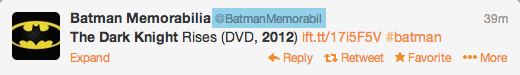
\includegraphics[width=4in]{image/tweet-user-field.png}
\centering
\caption{User name element (shown in blue) in a tweet retrieved by twitter web search}
\label{figure:tweet-user-field}
\end{figure}

\begin{lstlisting}[caption={HTML of the user name element in a tweet},label={user-name-element-html},captionpos=b]
  <span class=\"username js-action-profile-name\"><s>@</s><b>BatmanMemorabil</b></span>
\end{lstlisting}

\noindent
Using jQuery, a function can be created to count the occurances of the class "username js-action-profile-name", as shown in \ref{user-name-element-count-jquery-function}. This function can then be used to compare the number of user name elements in the DOM tree to the number of tweets in the search result, as shown in listing-\ref{user-elements-matches-tweets}. Since they are equal, it is likely that the right class is being scraped for the user name element.

\begin{lstlisting}[caption={Creating a function in GCDT Javascript Console for counting the occurance of user name elements on the twitter search result page},label={user-name-element-count-jquery-function},captionpos=b]
  > number_of_tweet_user_name_element_occurances = function(){ return $("span.username.js-action-profile-name").size() }
\end{lstlisting}


\begin{lstlisting}[caption={Running functions in GCDT Javascript Console to show that the number of user name elements matches the number of tweets},label={user-elements-matches-tweets},captionpos=b]
  > number_of_tweet_user_name_element_occurances();
  119
  > number_of_tweets_in_search_results();
  119
\end{lstlisting}

\subsubsection{User ID}
The user ID can also be found in the header. It is contained in the attribute data-user-id. Using the GCDT Select, it can be scraped from the page. It will be referred to as the user id element. The HTML of this scraping is shown in listing-\ref{listing:user-id-element-html}

\begin{lstlisting}[caption={HTML of the user id element in a tweet},label={listing:user-id-element-html},captionpos=b]
  <a class="account-group js-account-group js-action-profile js-user-profile-link js-nav" href="/username" data-user-id="userid">...</a>
\end{lstlisting}

\noindent
Using jQuery, a function can be created to count the occurances of the class used to specify the user id element, as shown in \ref{user-id-element-count-jquery-function}. This function can then be used to compare the number of user id elements in the DOM tree to the number of tweets in the search result, as shown in listing-\ref{user-id-elements-matches-tweets}. Since they are equal, it is likely that the right class is being scraped for the user id element.

\begin{lstlisting}[caption={Creating a function in GCDT Javascript Console for counting the occurance of user id elements on the twitter search result page},label={user-id-element-count-jquery-function},captionpos=b]
  > number_of_tweet_user_id_element_occurances = function(){ return $("a.account-group.js-account-group.js-action-profile.js-user-profile-link.js-nav").size() }
\end{lstlisting}

\begin{lstlisting}[caption={Running functions in GCDT Javascript Console to show that the number of user id elements matches the number of tweets},label={user-id-elements-matches-tweets},captionpos=b]
  > number_of_tweet_user_id_element_occurances();
  21
  > number_of_tweets_in_search_results();
  21
\end{lstlisting}

\subsubsection{Tweet Text}
The tweet text can be found in the content of the tweet, as shown in blue in figure-\ref{figure:tweet-text-field}. Using the GCDT Select, it can be extracted from the page. It will be referred to as the tweet content element. The tweet content element contains several HTML elements from which the text can be scraped, as shown in listing-\ref{listing:tweet-content-element-html}.

  \begin{figure}[H]
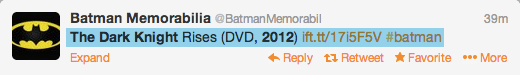
\includegraphics[width=4in]{image/tweet-text-and-url-field.png}
\centering
\caption{Tweet content element (shown in blue) in a tweet retrieved by twitter web search}
\label{figure:tweet-text-field}
\end{figure}

\begin{lstlisting}[caption={HTML of the tweet content element in a tweet},label={listing:tweet-content-element-html},captionpos=b]
  <p class="js-tweet-text tweet-text">
    <strong>The Dark Knight</strong> Rises (DVD, <strong>2012</strong>)
    <a href="http://t.co/p8pr9wqC4k" rel="nofollow" dir="ltr" data-expanded-url="http://ift.tt/17i5F5V" class="twitter-timeline-link" target="_blank" title="http://ift.tt/17i5F5V">
      <span class="tco-ellipsis"></span>
      <span class="invisible">http://</span>
      <span class="js-display-url">ift.tt/17i5F5V</span>
      <span class="invisible"></span>
      <span class="tco-ellipsis">
        <span class="invisible">&nbsp;</span>
      </span>
    </a>
    <a href="/search?q=%23batman&amp;src=hash" data-query-source="hashtag_click" class="twitter-hashtag pretty-link js-nav" dir="ltr">
      <s>#</s><b>batman</b>
    </a>
  </p>
\end{lstlisting}

\noindent
Using jQuery, a function can be created to count the occurances of the class "js-tweet-text tweet-text", which most likely describes all tweet content elements. The function is shown in listing-\ref{listing:tweet-content-element-count-function}. By comparing this number with the number of tweets in the search results and making sure it is equal, we can be confident that this class is describing the correct DOM element. The comparison is shown in
listing-\ref{listing:tweet-content-element-count-comparison}

\begin{lstlisting}[caption={Creating a function in GCDT Javascript Console for counting the occurance of tweet content elements on the twitter search result page},label={listing:tweet-content-element-count-function},captionpos=b]
  > number_of_tweet_content_element_occurances = function(){ return $("p.js-tweet-text.tweet-text").size() }
\end{lstlisting}

\begin{lstlisting}[caption={Running functions in GCDT Javascript Console to show that the number of tweet content elements matches the number of tweets},label={listing:tweet-content-element-count-comparison},captionpos=b]
  > number_of_tweet_content_element_occurances();
  119
  > number_of_tweets_in_search_results();
  119
\end{lstlisting}

\noindent
First, in order to obtain the tweet text, everything that is not a link or contained in a link must be scraped from the tweet content element in listing-\ref{listing:tweet-content-element-html}. An example of the HTML of this scraping is shown in listing-\ref{listing:tweet-text-scrape}. Then, the tweet text is obtained by stripping the HTML of all tags.

\begin{lstlisting}[caption={The HTML of scraping everything from listing-\ref{listing:tweet-content-element-html} that is not a link},label={listing:tweet-text-scrape},captionpos=b]
  <strong>The Dark Knight</strong> Rises (DVD, <strong>2012</strong>)
\end{lstlisting}

% End Twitter


% Start similar systems
\section{Similar Systems}\label{sec:similarsys}
In this section, similar systems will be discussed. Their usability in this project will also be evaluated.


\subsection{Recommender Systems}
\subsubsection{MovieLens}\label{subsec:MovieLens}
MovieLens is a movie recommendation system. A user creates an account and gets movie recommendations based on the user's own ratings through MovieLens' collaborative filtering algorithm. They use a item-item based algorithm. They take the 20 movies which are most similar to the target movie and see how these 20 movies where rated.\cite{grouplens}

The issue with using a strict item-item based correlation and the MovieLens recommendation system is that for a user with a low rating average, the user will very seldom get recommended movies with a top-average rating.


\subsubsection{MovieTweetings}\label{subsec:MovieTweetings}
MovieTweetings is an application for fetching movie ratings through the Twitter API from Twitter. The application search for ratings shared from IMDB, a movie information webpage, and stored. The user has the option of sharing the rating or not on Twitter, in the last case, the rating will not be caught by the MovieTweetings application.

With the use of a social media they wish to get a fresher dataset than using Netflix dataset, or MovieLens datasets~\ref{subsec:MovieLens}. At the time of writing the article they had more than 60 000 ratings, and about 500 new where added every day\cite{MovieTweetings}. The Twitter API is queried daily to update their database.

While querying the API for well structured tweets with ratings about movies are a good way to go when in search for a database with movie ratings, the data will be sparse. The data is not based on the users followers/followees, and will therefore not represent the social strength Twitter is capable of producing. A direct access to IMDB, rather than going through Twitter to get the rating information also seems like a simpler and more result-producing idea.


\subsubsection{Twittomender}
Twittomender is a followee recommender for Twitter. Twitter uses a friend's friend approach for recommending new Twitter-friends. This does not necessarily produce the most relevant recommendations for a user. Twittomender takes a collaborative approach to the problem. Tweets of a user are used and compare with other users tweets to to find similarities and recommend new Twitter-friendships\cite{twittomender}.

7 recommendation strategies, they are shown in table~\ref{table:to-strategies}.

\begin{table}[H]
\centering
\begin{tabular}{ l l }
  \textbf{Type} &  \textbf{Strategy} \\
  \hline \\ [-1.5ex]
  Content-based &  \pbox{20cm}{ (1) Users own tweets \\
                                (2) Followee’s tweets \\
                                (3) Follower’s tweets \\
                                (4) All tweets} \\
  \hline \\ [-1.5ex]
  Collaborative-based & \pbox{20cm}{  (5) Followee’s Ids \\
                                      (6) Follower’s Ids \\
                                      (7) All Ids }\\
  \hline \\ [-1.5ex]
\end{tabular}
\caption{The 7 recommendation strategies used by Twittomender}
\label{table:to-strategies}
\end{table}

The user interacts with the system through providing the system with their username on Twitter, the system produces a profile of the user based on tweets, and determines a score against other users based on most frequent terms amongst the users tweets. Each of the strategies are used from table~\ref{table:to-strategies} and top 20 from each are merged to a list where the most frequent users are returned as recommended users to explore for the user.

After testing on 1000 users the best performing strategy was a collaborative-based approach, users and follower connection, recommendation strategy (6).

What we can take from this is the strength of a user relationships.


\subsection{What the top Netflix-Prize contestants did}\label{subsec:thewinners}
\subsubsection{BellKor's Pragmatic Chaos}
BellKor's Pragmatic Chaos, the prize winners of the Netflix-Prize competition, was a group of scientists from AT\&T Labs, Yahoo!, Pragmatic Theory and Commendo Research \& Consulting. They achieved a RMSE of 0.8567, which was 10.06\% better than Netflix's own Cinematch score.

Models for the rating data is learned by fitting previously observed ratings, but since the model is to be used to predict feature ratings, overfitting the data. This achieved by regularizing the learned parameters. A regularization constant is used, and is set to L2 by default. This and other constant such as, step size and number of iterations are set manually through greedy manners. Where the algorithm is ran multiple times and constant value with best score is used. \cite{BellKor-CF-TD}

The winning algorithm was put together based on multiple different modeling techniques. Some of these modeling techniques are described below. \\\\


\textbf{Time of week rating}  The team saw that a user-rating done in the weekends had a tendency to have a higher value than a rating done on a Monday. This also applies for multiple ratings done the same day, higher ratings does not necessarily imply that the movie is much better than a movie rated lower another day, the user might just be in a good mood.

\textbf{Close User ratings}  Ratings done close to one another done by the same user implied that the user was rating based on the user's recollection of the rated movies, and not that the user just saw that movie, these ratings had to be handled in its own manner. This was because of the effect the faulty or old memories had on these ratings. The all time favorites/negatives are also usually in this bulk. While the movies which did not make much of an impression are forgotten. This helps us explain figure~\ref{figure:avgmovierating}, where we saw that movies with the edge ratings (1 or 5) had a lower rating distribution.

\textbf{Baseline predictors}  Some users has the tendency to rate on an overall average higher than other users.

\textbf{Movie like-ability}  Movies can go in and out of popularity. This change usually happens over a extended period.

\textbf{Frequency term}  The number of ratings a users gives on a specific day can help explains data-variability during that day.

\textbf{Matrix factorization with Temporal Dynamics (SVD)}  Single value decomposition use two sets pf static movie factors. Set one is used in all the models of the factors. Set two uses the movies rated by the user, normalizes the sum, and uses this as a user factor.

\textbf{Neighborhood model with Temporal Dynamics}  Most common approach to collaborative filtering. They used a item-item model based on global optimization. To predict rating of a new item based of rating an old item two sets of weights where used. One where the values of the ratings where accounted for, and one disregarding rating values.
A situation where a user rates an old item and a new item close to each other both in time and rating, is a better indicator that these items can be related to each other, than if two items are rated similarly, but with a greater timespan between each other.Therefore a decaying relationship is introduced between items. This decreased RMSE from 0.9002 to 0.8870.\cite{BellKor-CF-TD}

\textbf{Clustering}  In a cluster the average value is the predictor for the user/movie pairs in the cluster. Where the movie-set and user-set are divided randomly into 128 bins, and created $128*128=16384$ clusters. This was their only usage of clustering, they found that it had no measurable impact on the accuracy of the final blend\cite{pragmatictheory-sol}.

\textbf{Anchoring}  There is a order of when to watch some movies. For instance, some squeals are usually watched in the order they where made, and should be predicted that way. \\\\


Interestingly, the bias model with tanking in the factor that users change rating-scale over time, resulted in a RMSE of 0.9555, which is almost as good as the Cinematch Netflix was already using. The learning with the different modeling techniques is done by a stochastic gradient descent algorithm running for 30 iterations. This is the only time they use an automatic parameter tuner. \cite{BellKor-2008-sol}

The "BellKor's Pragmatic Chaos"-team used a lot of different models and did a lot of tweaking to get to the top. Some interesting findings to take from this is the importance of diversity and how central the timestamp of a rating can be.

\subsubsection{The Ensemble}
% http://www.the-ensemble.com/

A merger of the teams "Grand Prize Team" and "Opera Solutions and Vandelay United". They also managed to get a RMSE of 0.8567, and therefore a 10.09\% improvement as well. But lost since the "BellKor's Pragmatic Chaos"-team managed to submit their results 20 minutes earlier than "The Ensemble"-team.

The two merged teams, which made "The Ensemble" consisted of multiple smaller teams. They had all competed in the Netflix-Prize challenge, and had to put their heads and code together to get to the result they got to.

"The Ensemble"-team used a huge variation of models, just as the "BellKor's Pragmatic Chaos"-team.

After the competition was done "The Ensemble" tested a merger of their system with the "BellKor's Pragmatic Chaos"-system. The test RMSE of a 50/50 blend was 0.855476, which is a 10.19\% improvement. This is 0.10\% better then the teams managed to produce by themselves.

\subsubsection{Conclusion}
After looking at the two top contestants from the competition a pattern is starting to form. Diversity is key to be able to predict user-ratings at a top level.

While both the teams managed to produce a 10\% improvement over the original netflix algorithm, it was never taken into use~\cite{nfbeyond5}. Even though SVD and and RBM lowers the RMSE to 0.88 alone, are they not as applicable as wanted. The actual rating amount is 50 times bigger than the training set, and for SVD to give an accurate value, it has to be recalculated for each new rating, which is not applicable in a world where live recommendation is expected~\cite{nfbeyond5}.


\subsection{Recommender Algorithms}
\subsubsection{Probabilistic Neighborhood Selection}
A often used approach when recommending items is a neighborhood-based collaborative filtering. This approach often has the issue that it over-specializes and makes concentrated biases when recommending. When trying to estimate an unknown value, the nearest neighbors tend to produce a recommendation list with known items. The taste of the user is often multidimensional when it comes to movies, and these can be unknown to the k nearest neighbors to the user~\cite{umana}. This can be handled with a probabilistic approach when selecting neighbors~\cite{probcobfilter}. The approach does not estimate an unknown value based on the weighted averages of the k nearest neighbors, but rather on k probabilistically selected neighbors~\cite{optaplanner}. Another way of handling this issue is suggesting the least similar neighbors and their dislikes~\cite{furthestneighbor}. This approach was proved to be less accurate when calculating the RMSE~\cite{probcobfilter}, and will therefore not be explored further.

KNN is linear in the size of the training set, and therefore an efficient classification algorithm\cite{introtoIR}. And different implementations of it managed to produce RMSE scores from 0.91 to 1.002~\cite{knnnetflixstand, knnoldies, knnimpl, knncolbgroup}, even though K-NN has show to have some issues with sparse data~\cite{grobelnikDataSparsityIssues}, which implies that it will do better with a more complete dataset, which will be produced by the addition of social media data.


\subsubsection{Matrix Factorization}\label{subsubsec:matrixfac}
There are several matrix factorization algorithms. Amongst them single value decomposition (SVD) and alternating least squares (ALS) are valid candidates. As we saw from Bellkor's solution~\ref{subsec:thewinners} single value decomposition was used, and was a good addition to their blend. The issue with this algorithm is that it is rather computationally expensive and re-computation is needed to be done when new ratings are added, and therefore not very applicable to a live recommendation system. SVD performs well on sparse matrices, which the Netflix-dataset is~\cite{grobelnikDataSparsityIssues}.

ALS is a simpler and a very parallelizable matrix factorization algorithm, more so than SVD, but with many of the benefits that matrix factorization brings~\cite{predusingmatrix}. This makes it an interesting algorithm to look at.

This algorithm can be used to populate sparse matrices, just like the one from Netflix where the matrix is made up from users and movies. A rating matrix, $R$, is produced based on the use of two much smaller matrices. A number of "features" are set for each of the two smaller matrices $U$ and $M$, one for the users and one for the movies. The idea is to get $U^\top M$ as close to the real $R$. $U$ and $M$ are computed in two steps. This is easily parallelizable since solving for $U$ is independent of the other users, therefore the columns of $U$ can be computed in parallel. The information is gathered, and $M$ is updated, communication between movies is not necessary~\cite{myrrix}. With this algorithm a 0.9278 was produced, which is a 2\% improvement over Cinematch~\cite{predusingmatrix}. Runtime to produce this score was 2 hours on a high-end system~\cite{alsMPI}.


\subsection{Conclusion}\label{subsec:sim-sys-conc}
There are two basic problems when analyzing very large datasets: Writing the code correctly and the performance (i.e. speed at which it runs). As we saw from~\ref{subsubsec:matrixfac}, matrix factorization was one of the algorithms which preformed the best on the Netflix dataset. This is also shown in figure~\ref{figure:sub-distr-nf}. But the issue with it is if we want new ratings to be included in the recommendation system, then we need to recompute all recommendations, which is not ideally for a live recommendation system, where recommendation should include as much information as possible to be accurate.

The ALS~\ref{subsubsec:matrixfac} proved to be a very parallelizable algorithm, and a potential good alternative to SVD when doing live recommendation. But this requires a lot of computational power to make it live updating and will not be feasible to run on a low-end personal computer when wanting live results. But could prove to be a potential algorithm to use if one where to scale up to a high-end system.

The probabilistic neighborhood selection is a form of K-NN has a good runtime and produced a respectable RMSE. This is a well know approach to collaborative filtering, and there is a lot of documentations on different ways of selecting neighbors and implementation. This seems like the way to go as a start to produce recommendations on bigger datasets.
% end similar systems



\section{Development language and technologies}

\subsection{Database}
In order to easily retrieve data from the netflix prize dataset and store and retrieve data from twitter, it is useful to consider various kinds persistent storage or databases. There are three categories of options: Traditional file systems, SQL and NoSQL. Since traditional file systems are not designed for dynamically storing and retrieving data based on the structure of the data, they are not considered. The two options remaining are SQL and NoSQL which will be discussed and evaluated in the following sections.

\subsubsection*{NoSQL}
% http://en.wikipedia.org/wiki/NoSQL
NoSQL databases can be defined as: being non-relational. In many cases they are also: Open-source, distributed and horizontally scalable\cite{nosql}. NoSQL is meant for storing large amounts of data\cite{bigdata}, where all the data does not share the same attributes or schema. They are focusing on eventually consistency (BASE) instead of the more traditional consistent atomic transactions (ACID) \cite{pritchett}. The different kinds of NoSQL databases have different ways of classifying the database, some of the more used ones are: key-value, column, document, graph and relational.

\begin{table}[H]
\centering
\begin{adjustwidth}{-2cm}{}
\begin{tabularx}{1.3\textwidth}{  l l l l l l }
  \textbf{Data Model} & \textbf{Performance} & \textbf{Scalability} & \textbf{Flexibility} & \textbf{Complexity} & \textbf{Functionality}\\
  \hline \\ [-1.5ex]
  Key-value & high      & high              & high      & none      & variable (none)\\
  \hline \\ [-1.5ex]
  Column    & high      & high              & moderate  & low       & minimal \\
  \hline \\ [-1.5ex]
  Document  & high      & variable (high)   & high      & low       & variable (low)\\
  \hline \\ [-1.5ex]
  Graph     & variable  & variable          & high      & high      & graph theory \\
  \hline \\ [-1.5ex]
  Relational & variable & variable          & low       & moderate  & relational algebra\\
\end{tabularx}
\end{adjustwidth}
\caption{Differences in features of NoSQL Database Types}
\label{table:nosql-calssifications}
\end{table}
% http://www.slideshare.net/bscofield/nosql-death-to-relational-databases
As we can see from table~\ref{table:nosql-calssifications} performance, scalability and flexibility are usually rated as high in all the categories.

TODO: Move this to conclusion section
Relational algebra in the database will not be needed for the project to succeed so that category can be disregarded. High flexibility in the database would also be a feature sought after when going for NoSQL, so the column storage can also be eliminated from the equation. TODO: MAYBE SOMETHING MORE HERE lol the tree left are described well here : http://en.wikipedia.org/wiki/NoSQL
% http://en.wikipedia.org/wiki/Comparison_of_structured_storage_software
% http://www.mongodb.org/
\cite{nosql-databases, nosql-article}


\subsubsection*{SQL}
SQL databases are the most common way of storing structured data. The data is stored in columns and tables and is schema defined. This means that the attributes of the different datatypes are already defined and must be set whenever a datapoint is added to the database, even if it is NULL. The database can make relations between the tables id necessary, hence the name relational databases.
Performing queries is the way users and applications modify and read a SQL database. They are simple operations such as SELECT, UPDATE and DELETE written in the SQL query language. On a higher level of abstraction are transactions. Transactions are more or less a collection of queries. SQL Databases follow the ACID(atomicity, consistency, isolation, durability) principles for transactions. This means that the state of the database will never appear partially modified by a transaction to a new transaction that is being executed. Consistency of transactions are great for ensuring consistency across the data, but come at a performance cost.
\cite{ramakrishnan2003database}

\subsubsection{Database Alternatives}
Recommender systems are in nature performance heavy. They are also statistical which makes them fault tolerant. For this reason we have valued performance over consistency. The dataset is likely to have nested structure as it will combine two different types of data. Being able to append and combine data based on the structure of the content thus has value.
For these reasons the alternatives centered around NoSQL document stores, which are fast and have supports operations based on the structure of the document.
MySQL, which is the faster of the SQL alternatives, was also considered.

\subsubsection*{MongoDB}
MongoDB is a large scale, high availability, robust system. It is a NoSQL document store. Instead of storing the data in tables as in SQL, the data is stored in a BSON document. BSON stands for Binary JSON and is essentially a JSON document that is stored in binary instead of ASCII. A JSON document is a nested hash which can hold any number of attributes without depending on the other documents in the store. It is thus schemaless. Even though it is schemaless, MongoDB still possesses the some of the great properties from SQL databases, such as indexes, dynamic queries and updates.

MongoDB is implemented in C. It also has sharding which allows the database to scale horizontally. Custom queries and map-reduce queries can be written in JavaScript which has fast interpreters. This makes mongoDB an efficient and high speed data base for storing, modifying and fetching data with a nested document structure \cite{mongodb-intro}. In addition it has bindings to many different languages, which is a great advantage if some of the modules that need to access the database needs to be written in a language other than what it originally was written in.


\subsubsection*{CouchDB}
CouchDB is similar to MongoDB in the sense that it is a NoSQL Document store. It also has the same query capabilities as mongo and also uses JavaScript as a query language. In addition, CouchDB has a HTTP REST API which allows any web application to access it easily. CouchDB has a lot of built in features which makes web development with CouchDB easy. One of the greatest advantages is the intuitive web-based admin user-interface that is provided.
CouchDB does not support sharding which makes it less horizontally scalable. An alternative to achieve this is to use CouchBase, which is the distributed version of CouchDB. CouchDB is implemented in erlang. While erlang is faster than it used to be, it is certainly slower than a similar system written in pure C. In addition, CouchDB stores a copy of every single document every time it is modified. This makes CouchDB grow in size with time.
\cite{couchdb-about, couchdb-technical}


\subsubsection*{MySQL}
MySQL is one of the most popular database in the world of open databases. This is because of its high performance, reliability and ease of use. It should therefore be considered for the question of which database system to use. MySQL is an SQL based relational database, as opposed to the two NoSQL databases. It has bindings to most languages. It provides a much more advanced high level query language than a typical NoSQL document store. This is great for easily making complex queries during development, which is somewhat more tricky in NoSQL and JavaScript. However it is somewhat slower because of the interpretation of this high level language. The SQL database schema makes it more difficult to change the format of the data. MySQL also does not support JSON which is one of the most common standards for data retrieved from the web. This creates extra work with parsing JSON to the schema or invoking a mapper that has been created for this purpose.
\cite{mysql-about}


\subsubsection{Conclusion}
Even though MySQL has several of the properties needed for a recommendation system, it lacks the speed of a NoSQL store, which is a huge advantage. The complex join capabilities are not strictly necessary and can be replicated in JS in any of the two NoSQL document stores.

CouchDB has some unique merits. The simple web UI and HTTP REST API are great for development and compatability with web applications. However, compared to mongoDB it scores low on performance both as a standalone database, and in the sense that it can not be sharded to increase performance horizontally if necessary. It also takes up more space than necessary and grows in size for every single modification, which is an unfortunate property for a database that should handle a large fault tolerant dataset.

For these reasons mongoDB was chosen as the most appropriate alternative.


\subsection{Programming languages}
The main focus of our project is to harvest large amounts of data from the web, store it quickly in a database and do large computations on this data quickly. Because the design and implementation is likely to go through many iterations, it is important that the language chosen is most of all easy to modify. Performance of the language is also a valuable property.

\subsubsection{Ruby}
Ruby is a dynamic, interpreted, open source programming language with a focus on simplicity and productivity. Even though it is some times difficult to interpret ruby because there are always a large number of different ways to achieve the same functionarlity, ruby has an elegant syntax that is natural to read and easy to write. This is due to the fact that everything in Ruby is an object. Essential parts of Ruby can be removed or redefined, at will. Existing parts can be added upon. Ruby tries not to restrict the coder. This makes Ruby very flexible. \cite{ruby-about}

Ruby has one of the largest and most well crafted packaging systems of any language today. Packages in ruby are referred to as gems. RubyGems.org hosts more than 66000 gems to date. Gems can easily be created with the gem development tools that come with ruby. Gems also have very advanced yet simple requirement specification through Gemfiles. The name of required gems and ranges of working versions are specified in the Gemfile. All required gems can then be fetched with a single command. Creating a new gem or publishing a gem are also single commands. This makes managing dependencies and reusing code in ruby a breeze.\cite{rubygems}

Ruby is probably one of the most prevalent languages for modern web development. PHP is most likely still the most widely used, but ruby based web projects tend to be more managable due to the higher level frameworks and packages that are available.

\subsubsection{Python}
Python is a dynamic interpreted open source programming language. It is similar ruby in many ways. It has natural short typed syntax that is easy to read and write. For being an interpreted language, python is pretty fast. Python does not have an intuitive way of modifying existing parts of the language.\cite{python-about}

Python has a packaging system that is easy to use called Python Package Index, PIP for short. PIP hosts more than 37500 packages to date and has a very simple requirement specification and installation that only requires a few commands. This makes managing dependencies with python very easy.\cite{pip}

Python is widely used for a variety of cases. In particular science and web development. It also has some mature information retrieval libraries.

\subsubsection{Conclusion}
Python and Ruby are both great programming languages that fulfill the needs for writing modifiable code that can harvest and make predictions on data.

Python is slightly faster and has more mature information retrieval libraries. Ruby has more general packages available for reuse and is somewhat more modifiable.

The speed of python does not matter in the context of a web bottle neck. The algorithms in the information retrieval libraries must most likely be reimplemented to work with a database as these tend to do all predictions in memory. Because of this and because the authors have more experience with ruby, ruby was chosen over python.


\section{Result Testing}
Root-mean-square error (RMSE)~\ref{subsubsec:rmse} is a way of testing estimated value against the actual value. This is how they measured the correctness of the submitted solutions in the Netflix prize competition. To explore the correctness and improvement of the solution, this seems like a good way to go. The recommendation system will be ran on both the netflix-dataset alone and on the netflix-dataset merged with the twitter-data.

A reduction in the RMSE value will then indicate an improvement, and indicate the gain from the collaboration of movie data and social media data.

\section{Evaluation}\label{sec:prestrud-eval}
This section will sum up what we saw after doing the prestudy.

\subsection{Netflix}
The Netflix-dataset is very sparse. With about 480 000 users and 17 770 movies there would have been a total of more than 8.5 billion ratings, but the dataset only contains ca 100 million ratings, so algorithms which can handle this kind of sparsity must be used, such as alternating least squares and k nearest neighbors. The standard way to evaluate the correctness of a solution in these kinds of problems are RMSE.

\subsection{Twitter}\label{sec:prestrud-eval-twitter}
There are many different data types that can be retrieved from Twitter. The most dominating types and attributes are: Tweets, users, followees and followers.

There are several ways to access and retrieve this data. The REST API has the capability to retrieve the complete set of followees and followers for any given user. It lacks speed as it only allows 15 requests per 15 minute window.

The Streaming API is also great in the sense of data completeness. It has the capability of capturing all tweets for any given topic described by keywords. It is however slow in the sense that it takes a long time to build a dense dataset because less popular films are rarely tweeted about. In the study we see that even running the Stream API for over a year will only produce more than one tweet for about 65\% of the movies in the dataset. This is not satisfactory.

The Search API is great in the sense that it has looser limitations than the REST API. It can process a total of 180 requests per client per 15 minute window. It is however, like the Stream API limited in time span. The Search API only has a week worth of data. There is also no guarantee from Twitters side for which time window the Search API reflects and thus no guarantee for the completeness of data. This renders the Search API almost completely similar in terms of data gathering capability to the Stream API, but inferior in certainty of data completeness. A slight advantage for Search over Stream is that keeping a persistent connection is not required which makes it easier to maintain.

Scraping is the best solution in terms of data completeness and time consumption. It achieves what the Stream API is capable of achieving in years in mere days. However, it is a more complicated and error prone procedure as the scraping must be done by the client and the content being scraped is not under its control. The scraping procedure itself is more difficult to test than to just utilize an existing api. This makes Scraping more prone to sparseness and errors in the dataset. However, the speed with which an entire site can be crawled and scraped compared to the years it takes the Stream API to collect a dataset of the same density, makes it easy to test run a scraper, correct errors as they are found and run the scraper over again.

All of the previously mentioned APIs have the advantage that all the data gathered by them can be be aggregated and analyzed. Aggregations and analysis of data obtained by these means can be legally used to create services, including movie recommenders.

One problem with scraping is that it is not allowed by Twitter without their consent. As Twitters consent has not been granted to scrape Twitter for the purposes of this project, a dataset based on scraping can not be gathered. The data can certainly not be used to legally create services like movie recommenders.

All of the techniques for gathering data from Twitter discussed have pros and cons in terms of how dense of a dataset they build, how likely the dataset is to contain errors, how long they take to run and the legallity of how the data collection. As APIs exist for all techniques except scraping, the barrier for utilizing them are low. Implementing them and having them available has a low cost in terms of development time and each API increases the richness of available data. Implementing a scraper is also a good idea in case consent from Twitter is obtained as it has superior performance compared to any of the other techniques considered.

\subsection{Similar systems}
When it comes to recommendation systems it is important to weigh quality of result versus time it takes to produce this result. If it is too time-consuming the result might end up being outdated. Netflix did not implement the winner solution even though the winner managed to score 10\% better than the Netflix-system. This was mainly because of the time it took for the predictions to be calculated and Netflix need to have a live system.

TODO:fr Collaborative-based important, datasets utilizing user relationship like followers and followees tend to give the best results in twitter-based recommendations.

The group the user is a
For a big dataset and low computational time k nearest neighbors has proven to be a good way to go.
